\documentclass{article}
\usepackage{graphicx} % Required for inserting images

\title{Is Florida getting warmer?}
\author{Bridget Smith}
\date{December 2024}

\begin{document}

\maketitle

\section{Results}
I tested whether Florida is getting warmer, using the mean temperatures for each year in Florida from 1901 to 2000. I found the correlation coefficient between year and temperature to be 0.53. Since year and temperature are not independent variables, the significance of this correlation was tested by randomly permuting the temperature data and then finding a new correlation coefficient. This process was repeated 100,000 times. 

My null hypothesis is that there is no statistical effect of time on the average temperature in Florida. The approximate P-value is the fraction of correlation coefficients that are greater than 0.53. For a large sample, this value represents the probability of 0.53 being a correlation coefficient when the null hypothesis is true. For this data the approximate P-value is 0. Figure 1 shows the distribution of these shuffled correlation coefficients. The data is a symmetric bell-shaped curve centered around 0, so it is normally distributed.

This suggests that the null hypothesis should be rejected. There is a significant positive relationship between time and temperature in Florida in the twentieth century and indicating that Florida is getting warmer. 
\begin{figure}[h!]
    \centering
    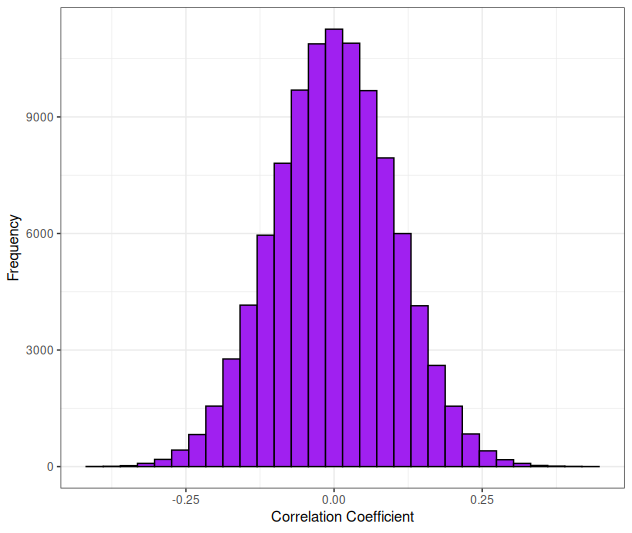
\includegraphics[width=0.5\linewidth]{../data/Rplot.png}
    \caption{A histogram of the correlation coefficients of each random shuffle of the temperature data.}
    \label{fig:enter-label}
\end{figure}
\end{document}
